

%----------------------------------------------------------------------------------------
%	PART
%----------------------------------------------------------------------------------------

\part{Capítulo cinco}

\graphicspath{ {img/ch5/}, {W_Varios/2_Portada_capitulos} }

%----------------------------------------------------------------------------------------
%	CHAPTER 5
%----------------------------------------------------------------------------------------

\chapterimage{5_Capitulo/img/portada/ima2} % Chapter heading image
\chapter{Series unif. diferidas, perpetuas y generales}
\section{Mapa Mental}
\begin{center}
	\includegraphics[scale=0.45]{5_Capitulo/img/explicacion/Mapa Mental 5.pdf}
\end{center}
\section{Fórmulas del capítulo}

\begin{spacing}{1.5}
	\begin{center}
		\begin{tabular}{ |p{4cm}|p{7cm}| p{3cm}|}
			\hline
			\rowcolor{orange!50}
			\begin{center}\textbf{Fórmula}\end{center}        & \begin{center}\textbf{Nombre}\end{center}                    & \begin{center} \textbf{Excel}\end{center} \\ \hline
			
			$VP = \frac{R}{i}$               & Valor presente serie perpetua vencida        & VA(i;10000;-R;;0)         \\ \hline
			$VP = R(\frac{1-(1+i)^{-n}}{i})$ & Valor presente de una serie uniforme vencida &                           \\ \hline
		\end{tabular}
	\end{center}
\end{spacing}

\section{Series uniformes diferidas}
Una serie uniforme es inmediata cuando el primer pago se encuentra en el primer período, si el pago se encuentra después de cierta cantidad de períodos se llama serie uniforme diferida: \\

\textbf{Ejemplo 1}\\
Para realizar un proyecto se necesita realizar una inversión inicial de 80.000 COP y otra inversión de
45.000 COP al final del primer mes, en los meses 2 y 3 los ingresos son equivalentes a los egresos;
pero a partir del mes 4, se producen ingresos así: Mes cuatro 30.000 COP, mes cinco 50.000 COP, mes
seis 60.000 COP. Determinar si el proyecto lo pueden realizar los inversionistas A o B mencionados
anteriormente.\\


%%%%%%%%%%%%%%%%%%% EJERCICIO 1 %%%%%%

%\newpage %USAR SOLO SI EL SOLUCION QUEDA SOLO Y ES NECESARIO BAJARLO A LA SIGUIENTE PAGINA
\textbf{Solución.}\\
%La tabla ira centrada
\begin{center}
	\renewcommand{\arraystretch}{1.5}% Margenes de las celdas
	%Creacion de la cuadricula de 3 columnas \end{flushleft}
	\begin{longtable}[H]{|C{0.3\linewidth}|C{0.3\linewidth}|C{0.3\linewidth}|}
		%Creamos una linea horizontal
		\hline
         %%%%% INICIO FLUJO DE CAJA
		\rowcolor[HTML]{FFB183}
		\multicolumn{3}{|c|}{\cellcolor[HTML]{FFB183}\textbf{1. Asignación periodo focal}}   \\ \hline
		\multicolumn{3}{|c|} {$pf = 0 pmv$} \\ \hline
		%%%%%%%%%% FIN TITULO
		%%%%%%%%%% INICIO TITULO
		%Lo que se hace aqui es mezclar las 3 columnas en una sola
		\multicolumn{3}{|c|}{\cellcolor[HTML]{FFB183}\textbf{2. Declaración de variables}}   \\ \hline
		%%%%%%%%%% FIN TITULO
		%%%%%%%%%% INICIO DE MATEMATICAS
		%Cada & hace referencia al paso de la siguiente columna
		$n_{0} = 0 pmv$   & $n_{1} = 1 pmv$ & $n_{2} =  4 pmv$\\
		$n_{3} = 5 pmv$ & $n_{4} = 6 pmv$ & \\ \hline
		\multicolumn{3}{|c|}{$i_{a} = TIO_{a} = 3\% \equiv 0.03 pmv$} \\
		\multicolumn{3}{|c|}{$i_{b} = TIO_{b} = 2\% \equiv 0.02 pmv$} \\ \hline
		%%%%%%%%%% FIN DE MATEMATICAS
		%%%%% FIN DECLARACION DE VARIABLES


		%%%%% INICIO FLUJO DE CAJA
		\rowcolor[HTML]{FFB183}
		\multicolumn{3}{|c|}{\cellcolor[HTML]{FFB183}\textbf{3. Diagrama de flujo de caja}} \\ \hline
		%Mezclamos 3 columnas y ponermos el dibujo
		%%%%%%%%%%%%% INSERCION DE LA IMAGEN
		%Deberan descargar las imagenes respectivas del drive y pegarlas en la carpeta
		%n_capitulo/img/ejemplos/1/capitulo1ejemplo1.pdf  (el /1/ es el numero del ejemplo)
		\multicolumn{3}{|c|}{ 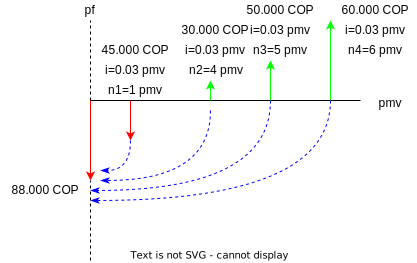
\includegraphics[trim=-5 -5 -5 -5 , scale=1.0,width=300px, height=250px]{9_Capitulo/ejemplos/1/Capitulo9Ejercicio1.pdf} }   \\ \hline
		%%%%%%%%%%%%% FIN INSERCION DE IMAGEN
		%%%%%FIN FLUJO DE CAJA



		%%%%% INICIO DECLARACION FORMULAS
		%%%%%%%%%%% INICIO TITULO
		\rowcolor[HTML]{FFB183}
		\multicolumn{3}{|c|}{\cellcolor[HTML]{FFB183}\textbf{4. Declaración de fórmulas}}    \\ \hline
		%%%%%%%%%%% FIN TITULO
		%%%%%%%%%%% INICIO MATEMATICAS
		\multicolumn{3}{|c|}{$\sum F_{n}(1+i)^{-n} $\hspace{0.3cm} \textit{Valor presente neto}} \\ \hline
		%%%%%%%%%% FIN MATEMATICAS
		%%%%%% INICIO DESARROLLO MATEMATICO
		\rowcolor[HTML]{FFB183}
		%%%%%%%%%%INICIO TITULO
		\multicolumn{3}{|c|}{\cellcolor[HTML]{FFB183}\textbf{5. Desarrollo matemático}}       \\ \hline
		%%%%%%%%%% FIN TITULO
		%%%%%%%%%% INICIO MATEMATICAS
		\multicolumn{3}{|c|}{$VPN_{a} = -80000 - 45000(1+0.03)^{-1} + 30000(1+0.03)^{-4} + 50000(1+0.03)^{-5} + 60000(1+0.03)^{-6}$} \\
		\multicolumn{3}{|c|}{$VPN_{a} = -3655$} \\
		\multicolumn{3}{|c|}{$VPN_{b} = -80000 - 45000(1+0.02)^{-1} + 30000(1+0.02)^{-4} + 50000(1+0.02)^{-5} + 60000(1+0.02)^{-6}$} \\
		\multicolumn{3}{|c|}{$VPN_{b} = 216254$} \\ \hline

		%%%%%%%%%% FIN MATEMATICAS
		%%%%%% FIN DESARROLLO MATEMATICO
		%%%%%% INICIO RESPUESTA
		\rowcolor[HTML]{FFB183}
		%%%%%%%%%%INICIO TITULO
		\multicolumn{3}{|c|}{\cellcolor[HTML]{FFB183}\textbf{6. Respuesta}}   \\ \hline
		%%%%%%%%%% FIN TITULO
		%%%%%%%%%% INICIO RESPUESTA MATEMATICA
		\multicolumn{3}{|c|}{Para B el $VPN > 0$, significa que puede realizar el proyecto en pesos de hoy,} \\ 
		\multicolumn{3}{|c|}{además de ganarse el 2\%, obtiene una ganancia de 2.162,54 COP.}  \\ \hline
		%%%%%%%%%% FIN MATEMATICAS
		%%%%%% FIN RESPUESTA
	\end{longtable}
	%Se crean dos lineas en blanco para que no quede el siguiente texto tan pegado
	%\newline \newline %USARLO SI CREES QUE ES NECESARIO
\end{center}
%%%%%%%%%%%%%%%%%%%%%%%%%%FIN EJERCICIO 1 %%%%%%%%%%%%%%%%%%%%%%%%%%%



\section{Series uniformes perpetuas}

Una serie uniforme que tiene infinito número de pagos se denomina serie uniforme perpetua. Una serie perpetua en la realidad no existe, ya que todo tiene su fin; se supone perpetua cuando el número de pagos o ingresos es muy grande o cuando no se sabe cuántos pagos son, pero se sospecha que son muchos.\\

Al deducir la fórmula de una serie uniforme vencida perpetua, debe tenerse en cuenta que solo existe el valor presente, porque el valor futuro de una serie uniforme vencida perpetua sería un valor bastante grande.\\

$ VP = \lim_{n\to \infty}R\frac{1-(1+i)^{-n}}{i} = \lim_{n\to \infty} R\frac{1-0}{i} = \frac{R}{i}$\\

$ VP = \frac{R}{i}$ \hspace{35pt}\textit{Valor presente de una serie uniforme vencida perpetua}\\ \\

\textbf{Ejemplo 2}\\
Se invierten 200{.}000 COP en un depósito a término fijo de 6 meses en un banco que paga el 28\% namv. Determinar el monto de la entrega al vencimiento.\\

%%%%%%%%%%%%%%%%%%% EJERCICIO 1 %%%%%%

%\newpage %USAR SOLO SI EL SOLUCIÓN QUEDA SOLO Y ES NECESARIO BAJARLO A LA SIGUIENTE PAGINA
\textbf{Solución.}
%La tabla ira centrada
\begin{center}
  \renewcommand{\arraystretch}{1.5}% Margenes de las celdas
  %Creación de la cuadricula de 3 columnas \end{flushleft}
  \begin{longtable}[H]{|C{0.3\linewidth}|C{0.3\linewidth}|C{0.3\linewidth}|}
    %Creamos una linea horizontal
    \hline
    %Definimos el color de la primera fila
    \rowcolor[HTML]{FFB183}
    %%%%% INICIO ASIGNACIÓN FECHA FOCAL %%%%%%%
    %%%%%%%%%% INICIO TITULO
    %Lo que se hace aquí es mezclar las 3 columnas en una sola
    \multicolumn{3}{|c|}{\cellcolor[HTML]{FFB183}\textbf{1. Asignación período focal}}                                  \\ \hline
    %%%%%%%%%% FIN TITULO
    %%%%% INICIO DECLARACIÓN DE VARIABLES %%%%%%%
    \multicolumn{3}{|c|}{$pf = 6pmv$}                                                                                   \\ \hline
    %%%%%%%%%% INICIO TITULO
    %Lo que se hace aquí es mezclar las 3 columnas en una sola
    \multicolumn{3}{|c|}{\cellcolor[HTML]{FFB183}\textbf{2. Declaración de variables}}                                  \\ \hline
    %%%%%%%%%% FIN TITULO
    %%%%%%%%%% INICIO DE MATEMÁTICAS
    %Cada & hace referencia al paso de la siguiente columna
    $P =  200{.}000$ COP & $n = 6\textit{pmv} $ & $i= ?\% pmv$                                                           \\
    $j=28\%namv$         & $m=12pmv$            & $F = ? COP$                                                           
    \\\hline

    %%%%%%%%%% FIN DE MATEMÁTICAS
    %%%%% FIN DECLARACIÓN DE VARIABLES


    %%%%% INICIO FLUJO DE CAJA
    \rowcolor[HTML]{FFB183}
    \multicolumn{3}{|c|}{\cellcolor[HTML]{FFB183}\textbf{3. Diagrama de flujo de caja}}                                 \\ \hline
    %Mezclamos 3 columnas y pondremos el dibujo
    %%%%%%%%%%%%% INSERCIÓN DE LA IMAGEN
    %Deberán descargar las imágenes respectivas del drive y pegarlas en la carpeta
    %n_capitulo/img/ejemplos/1/capitulo1ejemplo1.pdf  (el /1/ es el numero del ejemplo)
    \multicolumn{3}{|c|}{ 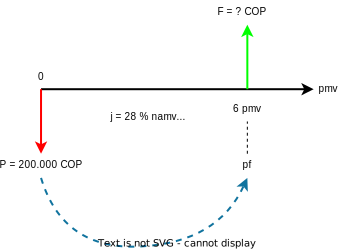
\includegraphics[trim=-5 -5 -5 -5 , scale=1]{2_Capitulo/ejemplos/2/Capitulo2Ejercicio2_v2.pdf} } \\ \hline
    %%%%%%%%%%%%% FIN INSERCIÓN DE IMAGEN
    %%%%%FIN FLUJO DE CAJA



    %%%%% INICIO DECLARACIÓN FORMULAS
    %%%%%%%%%%% INICIO TITULO
    \rowcolor[HTML]{FFB183}
    \multicolumn{3}{|c|}{\cellcolor[HTML]{FFB183}\textbf{4. Declaración de fórmulas}}                                   \\ \hline
    %%%%%%%%%%% FIN TITULO
    %%%%%%%%%%% INICIO MATEMÁTICAS
    \multicolumn{3}{|c|}{$F = P(1+i)^n \hspace{0.3cm} \textit{Valor futuro}$}                                           \\
    \multicolumn{3}{|c|}{$j=i\cdot m\hspace{0.3cm}\textit{Tasa periódica anualizada}$}
    \\ \hline
    %%%%%%%%%% FIN MATEMÁTICAS
    %%%%%% INICIO DESARROLLO MATEMÁTICO
    \rowcolor[HTML]{FFB183}
    %%%%%%%%%%INICIO TITULO
    \multicolumn{3}{|c|}{\cellcolor[HTML]{FFB183}\textbf{5. Desarrollo matemático}}                                     \\ \hline
    %%%%%%%%%% FIN TITULO
    %%%%%%%%%% INICIO MATEMÁTICAS
    \multicolumn{3}{|c|}{$0{.}28=i\cdot 12$}                                                                            \\
    \multicolumn{3}{|c|}{$i= \frac{0{.}28}{12} = 0{.}02333... \equiv 2{.}333\%pmv$}                                     \\
    \multicolumn{3}{|c|}{$0{.}28=i\cdot 12$}                                                                            \\
    \multicolumn{3}{|c|}{$F = 200{.}000 COP(1+0,2333)^6$}                                                       \\
    \multicolumn{3}{|c|}{$F = 229{.}685.04 COP$}
    \\ \hline


    %%%%%%%%%% FIN MATEMÁTICAS
    %%%%%% FIN DESARROLLO MATEMÁTICO
    %%%%%% INICIO RESPUESTA
    \rowcolor[HTML]{FFB183}
    %%%%%%%%%%INICIO TITULO
    \multicolumn{3}{|c|}{\cellcolor[HTML]{FFB183}\textbf{6. Respuesta}}                                                 \\ \hline
    %%%%%%%%%% FIN TITULO
    %%%%%%%%%% INICIO RESPUESTA MATEMÁTICA
    \multicolumn{3}{|c|}{$F = 229{.}685.04 COP$
    }                                                                                                                   \\ \hline
    %%%%%%%%%% FIN MATEMÁTICAS
    %%%%%% FIN RESPUESTA
  \end{longtable}
  %Se crean dos lineas en blanco para que no quede el siguiente texto tan pegado
  %\newline \newline %USARLO SI CREES QUE ES NECESARIO
\end{center}
%%%%%%%%%%%%%%%%%%%%%%%%%%FIN EJERCICIO 1 %%%%%%%%%%%%%%%%%%%%%%%%%%%



\section{Series uniformes generales}

Una serie uniforme simple es aquella donde el período de interés coincide con el período de pago. Por el contrario en una serie uniforme general el período de pago no coincide con el período de interés, por ejemplo, una serie de pagos trimestrales con una tasa periódica semestral.\\

Una serie uniforme general puede ser reducida a una serie uniforme simple, si hacemos que los períodos de tiempo y los períodos de interés coincidan. Hay dos formas para realizarlo:\\

\begin{enumerate}
	\item Encontrar el valor de pagos que se hicieron al final de cada período de interés y sean equivalentes al pago único que se hace al final de un período de pago.
	\item Cambiar la tasa usando tasas de equivalencia, dando lugar a que coincidan los períodos de interés y de pago.\\
\end{enumerate}

\textbf{Ejemplo 3}\\
Una fabrica produce actualmente en forma manual 1.000 unidades de un determinado artículo, para ello utiliza artesanos a los cuales les paga 8.400.000 COP al año y, es costumbre que cada año se les aumente el sueldo en aproximadamente un 20\%. El precio de venta de cada artículo es de 9.000 COP y se estima que este precio podrá ser aumentado todos los años en un 21\%. Ahora se ha presentado la oportunidad de adquirir una máquina a un costo de 10 millones COP con una vida útil de 5 años; un valor de salvamento de 2 millones COP la cual requiere de 2 técnicos para su operación, el sueldo anual de cada uno de los técnicos puede ser de 600.000 COP con aumentos anuales de sueldo del 20\% ¿Cuál de las dos alternativas es mejor suponiendo que la tasa del inversionista es del 30\%?\\


%%%%%%%%%%%%%%%%%%% EJERCICIO 3 %%%%%%

%\newpage %USAR SOLO SI EL SOLUCION QUEDA SOLO Y ES NECESARIO BAJARLO A LA SIGUIENTE PAGINA
\textbf{Solución.}\\
%La tabla ira centrada
\begin{center}
	\renewcommand{\arraystretch}{1.5}% Margenes de las celdas
	%Creacion de la cuadricula de 3 columnas \end{flushleft}
	\begin{longtable}[H]{|C{0.3\linewidth}|C{0.3\linewidth}|C{0.3\linewidth}|}
		%Creamos una linea horizontal
		\hline
        %%%%% INICIO FLUJO DE CAJA
		\rowcolor[HTML]{FFB183}
		\multicolumn{3}{|c|}{\cellcolor[HTML]{FFB183}\textbf{1. Asignación periodo focal}}   \\ \hline
		\multicolumn{3}{|c|} {$pf = 0 pav$} \\ \hline
		%%%%%%%%%% FIN TITULO
		%%%%%%%%%% INICIO TITULO
		%Lo que se hace aqui es mezclar las 3 columnas en una sola
		\multicolumn{3}{|c|}{\cellcolor[HTML]{FFB183}\textbf{2. Declaración de variables}}   \\ \hline
		%%%%%%%%%% FIN TITULO
		%%%%%%%%%% INICIO DE MATEMATICAS
		%Cada & hace referencia al paso de la siguiente columna
		$R_{1} = 9.000.000 $ COP   & $R_{2} = 8.400.000$ COP  & $i=0.3pav$\\ 
		$g_{1} =  0.21 pav $ & $g_{2}=  0.2 pav $ & $n=5pav$ \\ \hline
		%%%%%%%%%% FIN DE MATEMATICAS
		%%%%% FIN DECLARACION DE VARIABLES

  		%%%%% INICIO DECLARACION FORMULAS
  
		%%%%%%%%%%% INICIO TITULO
		\rowcolor[HTML]{FFB183}
		\multicolumn{3}{|c|}{\cellcolor[HTML]{FFB183}\textbf{3. Diagrama de flujo de caja}} \\ \hline
		%Mezclamos 3 columnas y ponermos el dibujo
		%%%%%%%%%%%%% INSERCION DE LA IMAGEN
		%Deberan descargar las imagenes respectivas del drive y pegarlas en la carpeta
		%n_capitulo/img/ejemplos/1/capitulo1ejemplo1.pdf  (el /1/ es el numero del ejemplo)
		\multicolumn{3}{|c|}{ \includegraphics[trim=-5 -5 -5 -5 , scale=1, width=300px, height=250px]{9_Capitulo/ejemplos/3/Capitulo9Ejercicio3.pdf} }   \\ \hline
		%%%%%%%%%%%%% FIN INSERCION DE IMAGEN
		%%%%%FIN FLUJO DE CAJA



		%%%%% INICIO DECLARACION FORMULAS
		%%%%%%%%%%% INICIO TITULO
		\rowcolor[HTML]{FFB183}
		\multicolumn{3}{|c|}{\cellcolor[HTML]{FFB183}\textbf{4. Declaración de fórmulas}}    \\ \hline
		%%%%%%%%%%% FIN TITULO
		%%%%%%%%%%% INICIO MATEMATICAS
		\multicolumn{3}{|c|}{$\sum F_{n}(1+i)^{-n} $\hspace{0.3cm} \textit{Valor presente neto}} \\ \hline
		%%%%%%%%%% FIN MATEMATICAS
		%%%%%% INICIO DESARROLLO MATEMATICO
		\rowcolor[HTML]{FFB183}
		%%%%%%%%%%INICIO TITULO
		\multicolumn{3}{|c|}{\cellcolor[HTML]{FFB183}\textbf{5. Desarrollo matemático}}       \\ \hline
		%%%%%%%%%% FIN TITULO
		%%%%%%%%%% INICIO MATEMATICAS
		\multicolumn{3}{|c|}{$VPN_{A} = \frac{9[(1+0.21)^{5}(1+0.3)^{-5} -1]}{0.21-0.3} - \frac{8.4[(1+0.2)^{5}(1+0.3^{-5} -1)]}{0.2-0.3}$} \\
		\multicolumn{3}{|c|}{$VPN_{A} = 2.437.836 $ COP} \\
		\multicolumn{3}{|c|}{$VPN_{B} = \frac{9[(1+0.21)^{5}(1+0.3)^{-5} -1]}{0.21-0.3} + 2(1.3)^{-5} - \frac{1.2[(1+0.2)^{5}(1+0.3^{-5} -1)]}{0.2-0.3}$} \\
		\multicolumn{3}{|c|}{$VPN_{B} = 16.723.756 $ COP} \\ \hline

		%%%%%%%%%% FIN MATEMATICAS
		%%%%%% FIN DESARROLLO MATEMATICO
		%%%%%% INICIO RESPUESTA
		\rowcolor[HTML]{FFB183}
		%%%%%%%%%%INICIO TITULO
		\multicolumn{3}{|c|}{\cellcolor[HTML]{FFB183}\textbf{6. Respuesta}}   \\ \hline
		%%%%%%%%%% FIN TITULO
		%%%%%%%%%% INICIO RESPUESTA MATEMATICA
		\multicolumn{3}{|c|}{La decisión correcta es comprar la máquina.}  \\ \hline
		%%%%%%%%%% FIN MATEMATICAS
		%%%%%% FIN RESPUESTA
	\end{longtable}
	%Se crean dos lineas en blanco para que no quede el siguiente texto tan pegado
	%\newline \newline %USARLO SI CREES QUE ES NECESARIO
\end{center}
%%%%%%%%%%%%%%%%%%%%%%%%%%FIN EJERCICIO 3 %%%%%%%%%%%%%%%%%%%%%%%%%%%


\newpage

\textbf{Ejemplo 4:}\\
Una entidad estatal puede usar el edificio A que requiere 5.000.000 COP cada año como costo de mantenimiento y  6.000.000 COP cada 5 años para reparaciones, o puede usar el edificio B, que requiere  5.100.000 COP cada año como costo de funcionamiento y  1.000.000 COP cada 2 años para reparaciones. Suponiendo una tasa de $j=30\%$ nominal anual año vencido y que el edifico escogido se ocupara por tiempo indefinido, ¿cuál de los dos edificios le resulta más conveniente utilizar?\\

\textbf{Solución:}

%La tabla ira centrada
\begin{center}
 \renewcommand{\arraystretch}{1.5}% Margenes de las celdas
 %Creación de la cuadricula de 3 columnas
 \begin{longtable}[H]{|c|c|c|}
  %Creamos una linea horizontal
  \hline
  %Definimos el color de la primera fila
  \rowcolor[HTML]{FFB183}
  %%%%% INICIO ASIGNACIÓN FECHA FOCAL %%%%%%%
  %%%%%%%%%% INICIO TITULO
  %Lo que se hace aquí es mezclar las 3 columnas en una sola
  \multicolumn{3}{|c|}{\cellcolor[HTML]{FFB183}\textbf{1. Asignación período focal}}\\ \hline
  \multicolumn{3}{|c|} {$pf=0\textit{ pav}$}\\ \hline
  %%%%%%%%%% FIN TITULO
  %%%%% INICIO DECLARACIÓN DE VARIABLES %%%%%%%
  %%%%%%%%%% INICIO TITULO
  %Lo que se hace aquí es mezclar las 3 columnas en una sola
  \multicolumn{3}{|c|}{\cellcolor[HTML]{FFB183}\textbf{2. Declaración de variables}}\\ \hline
  %%%%%%%%%% FIN TITULO
  %%%%%%%%%% INICIO DE MATEMÁTICAS
  %Cada & hace referencia al paso de la siguiente columna
  \multicolumn{2}{|l|}{$R_{a_1}=5{.}000{.}000\,\,COP\textit{ matenimiento cada año}$} & $VP_a= ?\,\,COP$   \\
  \multicolumn{2}{|l|}{$R_{a_2}=6{.}000{.}000\,\,COP\textit{ reparacion cada 5 años}$} & $VP_b= ?\,\,COP$   \\
  \multicolumn{2}{|l|}{$R_{b_1}=5{.}100{.}000\,\,COP\textit{ matenimiento cada año}$} & \\
  \multicolumn{2}{|l|}{$R_{b_2}=1{.}000{.}000\,\,COP\textit{ reparación cada 2 años}$} & \\ \hline
  
  %%%%% INICIO FLUJO DE CAJA
  \rowcolor[HTML]{FFB183}
  \multicolumn{3}{|c|}{\cellcolor[HTML]{FFB183}\textbf{3. Diagrama de flujo de caja}}
  \\ \hline
  %Mezclamos 3 columnas y pondremos el dibujo
  %%%%%%%%%%%%% INSERCIÓN DE LA IMAGEN
  %Deberán descargar las imágenes respectivas del drive y pegarlas en la carpeta
  %n_capitulo/img/ejemplos/1/capitulo1ejemplo1.pdf  (el /1/ es el numero del ejemplo)
  \multicolumn{3}{|c|}{ \includegraphics[trim=-5 -5 -5 -5 , max width=250px, max height=350px]{5_Capitulo/ejemplos/4/Capitulo5Ejemplo4-1.pdf} }\\
  \multicolumn{3}{|c|}{ \includegraphics[trim=-5 -5 -5 -5 , max width=250px, max height=350px]{5_Capitulo/ejemplos/4/Capitulo5Ejemplo4-2.pdf} }\\
  \hline
  %%%%%%%%%%%%% FIN INSERCIÓN DE IMAGEN
  %%%%%FIN FLUJO DE CAJA  
  
  %%%%% INICIO DECLARACIÓN FORMULAS
  %%%%%%%%%%% INICIO TITULO
  \rowcolor[HTML]{FFB183}
  \multicolumn{3}{|c|}{\cellcolor[HTML]{FFB183}\textbf{4. Declaración de fórmulas}}\\ \hline
  %%%%%%%%%%% FIN TITULO
  %%%%%%%%%%% INICIO MATEMÁTICAS
  
  \multicolumn{3}{|c|}{$VF=R(\frac{(1+i)^n-1}{i}) \hspace{0.4 cm} \textit{Valor futuro de una serie uniforme vencida}$}\\
  \multicolumn{3}{|c|}{$VP=\frac{R}{i} \hspace{0.4 cm} \textit{Valor presente de una serie uniforme vencida perpetua}$}\\
  \hline
  
  %%%%%%%%%% FIN MATEMÁTICAS
  %%%%%% INICIO DESARROLLO MATEMÁTICO
  \rowcolor[HTML]{FFB183}
  %%%%%%%%%%INICIO TITULO
  \multicolumn{3}{|c|}{\cellcolor[HTML]{FFB183}\textbf{5. Desarrollo matemático}}\\ \hline
  %%%%%%%%%% FIN TITULO
  %%%%%%%%%% INICIO MATEMÁTICAS
  \multicolumn{3}{|l|}{\textbf{Para el edificio A:}}\\
  \multicolumn{3}{|p{\textwidth}|}{Cálculo del valor presente de la serie uniforme vencida perpetua del costo anual de mantenimiento:}\\
  \multicolumn{3}{|c|}{$VP_{a_1}=\frac{5{.}000{.}000\,\,COP}{0.3\,pav}\hspace{0.2 cm}\rightarrow \hspace{0.2 cm}VP_{a_1}=16{.}666{.}666.67\,\,COP$}\\
  \multicolumn{3}{|p{\textwidth}|}{Cálculo de la R anual equivalente de la serie quinquenal de reparación.}\\
  \multicolumn{3}{|c|}{$6{.}000{.}000\,\,COP=R_{R_{a2}}(\frac{(1+0.3)^5-1}{0.3})\hspace{0.2 cm}\rightarrow \hspace{0.2 cm}R_{R_{a2}}=663{.}489\,\,COP$} \\
  \multicolumn{3}{|p{\textwidth}|}{Cálculo del valor presente de la serie uniforme vencida anual perpetua equivalente por la reparación.}\\
  \multicolumn{3}{|c|}{$VP_{a_2}=\frac{663{.}490\,\,COP}{0.3}\hspace{0.2 cm}\rightarrow \hspace{0.2 cm}VP_{a_2}=2{.}211{.}631\,\,COP$}\\
  \multicolumn{3}{|c|}{$VP_{a}=16{.}666{.}667\,\,COP+2{.}211{.}631\,\,COP\hspace{0.2 cm}\rightarrow \hspace{0.2 cm}VP_{a}=18{.}878{.}798\,\,COP$}\\
  \multicolumn{3}{|l|}{\textbf{Para el edificio B:}}\\
  \multicolumn{3}{|p{\textwidth}|}{Se repiten los mismos cálculos:}\\
  \multicolumn{3}{|c|}{$VP_{a_1}=\frac{5{.}100{.}000\,\,COP}{0.3}\hspace{0.2 cm}\rightarrow \hspace{0.2 cm}VP_{b_1}=17{.}000{.}000\,\,COP$}\\
  \multicolumn{3}{|c|}{$1{.}000{.}000\,\,COP=R_{R_{b2}}(\frac{(1+0.3)^2-1}{0.3})\hspace{0.2 cm}\rightarrow \hspace{0.2 cm}R_{R_{b2}}=434{.}783\,\,COP$} \\
  \multicolumn{3}{|c|}{$VP_{b_2}=\frac{434{.}783\,\,COP}{0.3}\hspace{0.2 cm}\rightarrow \hspace{0.2 cm}VP_{b_2}=1{.}449{.}275\,\,COP$}\\
  \multicolumn{3}{|c|}{$VP_{b}=17{.}000{.}000\,\,COP+1{.}449{.}275\,\,COP\hspace{0.2 cm}\rightarrow \hspace{0.2 cm}VP_{b}=18{.}449{.}275\,\,COP$}\\
  \multicolumn{3}{|c|}{$VP_a-VP_b=18{.}878{.}798\,\,COP-18{.}449{.}275\,\,COP=429{.}522\,\,COP\hspace{0.2 cm}$}\\
  \hline

  %%%%%%%%%% FIN MATEMÁTICAS
  %%%%%% FIN DESARROLLO MATEMÁTICO
  %%%%%% INICIO RESPUESTA
  \rowcolor[HTML]{FFB183}
  %%%%%%%%%%INICIO TITULO
  \multicolumn{3}{|c|}{\cellcolor[HTML]{FFB183}\textbf{6. Respuesta}}\\
  \hline
  %%%%%%%%%% FIN TITULO
  %%%%%%%%%% INICIO RESPUESTA MATEMÁTICA
  \multicolumn{3}{|p{\textwidth}|}{\centering{Es conveniente hacer uso del edificio B, que representa un ahorro de $429{.}522\,\,COP$}}
  \\ \hline
  %%%%%%%%%% FIN MATEMÁTICAS
  %%%%%% FIN RESPUESTA
 \end{longtable}
 %Se crean dos lineas en blanco para que no quede el siguiente texto tan pegado
 %\newline \newline %USARLO SI CREES QUE ES NECESARIO
\end{center}
%%%%%%%%%%%%%%%%%%%%%%%%%%FIN EJERCICIO 4 %%%%%%%%%%%%%%%%%%%%%%%%%%%


%----------------------------------------------------------------------------------------
%	PART
%----------------------------------------------------------------------------------------

%\part{Parte Dos}

%----------------------------------------------------------------------------------------
%	CHAPTER 3
%----------------------------------------------------------------------------------------

%\chapterimage{ima2} % Chapter heading image


%Anexos
%\chapter*{Anexos}
%\addcontentsline{toc}{chapter}{\textcolor{ocre}{Anexos}}




%----------------

%----------------------------------------------------------------------------------------
%	BIBLIOGRAPHY
%----------------------------------------------------------------------------------------

%\chapter*{Bibliografía}
%\addcontentsline{toc}{chapter}{\textcolor{ocre}{Bibliografía}}
%\section*{Books}
%\addcontentsline{toc}{section}{Books}
%\printbibliography[heading=bibempty,type=book]



%----------------------------------------------------------------------------------------
%	INDEX
%----------------------------------------------------------------------------------------

\cleardoublepage
\phantomsection
\setlength{\columnsep}{0.75cm}
\printindex

%----------------------------------------------------------------------------------------
